% Prof. Dr. Ausberto S. Castro Vera
% UENF - CCT - LCMAT - Curso de Ci\^{e}ncia da Computa\c{c}\~{a}o
% Campos, RJ,  2021
% Disciplina: Paradigmas de Linguagens de Programa\c{c}\~{a}o
%


\chapter{ Conceitos básicos da Linguagem Julia}

Neste capítulo apresentamos os conceitos basais de sintaxe, design e ferramental necessários para se programar em Julia. Para tanto, nos baseamos nos três principais livros-texto voltados ao estudo da linguagem, com destaque para \cite{Lobianco2019}, seguido de \cite{Lauwens2019} e \cite{Kwong2020}.

\section{Preparação do ambiente}
%Faltando algo para conectar esse parágrafo ao anterior []
Para executar código Júlia, basta baixar e descompactar os arquivos binários no site oficial da linguagem. O arquivo executável apresenta o console de interpretação mostrado na figura \ref{REPL} (também conhecido como "REPL - Read, Eval, Print, Loop") por onde é possível executar Julia tanto por linha de comando quanto por meio de scripts .jl. Também é possível utilizar diversos ambientes de desenvolvimento integrado que serão abordados alguns capítulos adiante.
%Deveria colocar esse parágrafo em uma nova section? tipo first things first? []
\begin{figure}[H]
\begin{center}
    \caption{REPL Julia} \label{REPL}
    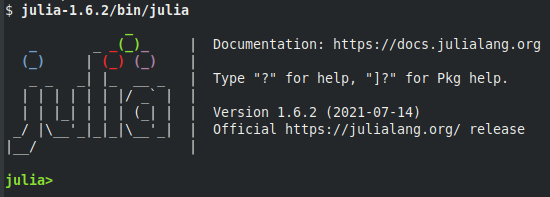
\includegraphics[width=12cm]{aplicacoes/ambiente.png} \\
    {\tiny \sf Fonte: Autor}
\end{center}
\end{figure} 

\section{Considerações gerais sobre sintaxe}
A seguir listamos alguns pontos importantes da sintaxe de Julia. 
%Adicionar exemplos em código? []
\begin{itemize}
    \item Podemos adicionar ao código comentários de uma linha (\#) ou de múltiplas linhas (\#= =\#) que podem ser aninhados e colocados em qualquer lugar como mostra a figura \ref{comentarios}.

    \item Blocos não precisam de parênteses, utilizamos a palavra "end" para indicar o fim de um bloco, conforme figura \ref{blocos_identacao}.
    \item Espaços são sintaticamente significantes, identação, não. (Fig \ref{blocos_identacao}).
    \item Nomes de variáveis aceitam um subconjunto dos simbolos Unicode como letras gregas e até emojis. (Fig \ref{emoji})
    \item Vetores iniciam com o índice 1. (Fig \ref{indice})
    \item Por convenção, funções que podem alterar algum de seus argumentos têm um ponto de exclamação (!) no fim de seu nome. A função de ordenação (sort), por exemplo, recebe um vetor V desordenado e tem duas possibilidades: a função sort(V) retorna um vetor com os elementos de V ordenados, sem alterar o vetor V. Já a função sort!(V) ordena o próprio vetor, sem retorno. Podemos observar essa diferença na figura \ref{exclamacao}.
    \item O ponto e vírgula (;) é utilizado para suprimir o output de um comando ou acessar o shell (a partir do REPL) como apresentado na figura \ref{supressao}.
    
  \end{itemize}
    
    \begin{figure}[H]%comentarios
    \begin{center}
        \label{comentarios}
        \caption{Comentários em Julia} 
        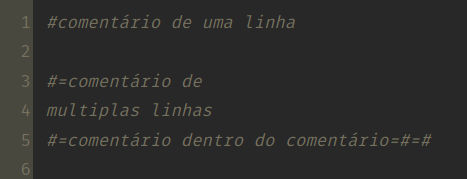
\includegraphics[width=12cm]{aplicacoes/comentarios.png} \\
        {\tiny \sf Fonte: Autor}
    \end{center}
    \end{figure} 

    \begin{figure}[H]%blocos
    \begin{center}
        \label{blocos_identacao}
        \caption{Blocos e identação em Julia} 
        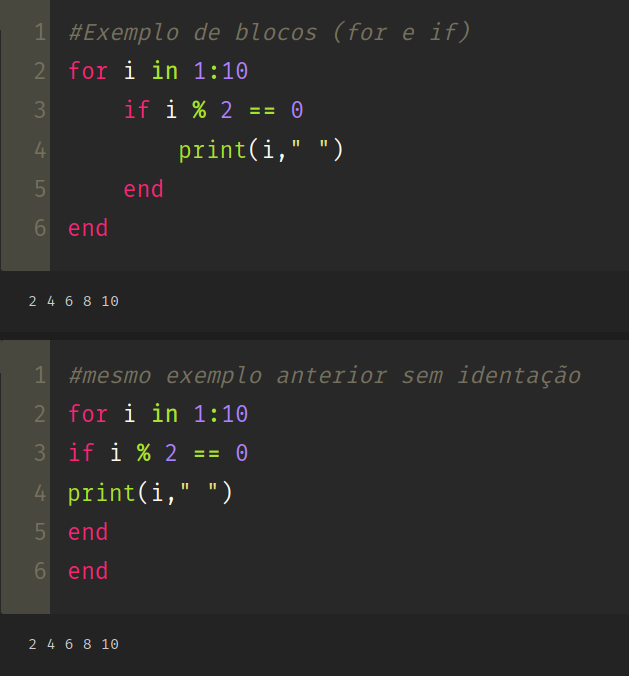
\includegraphics[width=12cm]{aplicacoes/bloco_identacao.png} \\
        {\tiny \sf Fonte: Autor}
    \end{center}
    \end{figure} 

%    \begin{figure}[H]%identacao
%    \begin{center}
%        \label{identacao}
%        \caption{Identação em Julia} 
%        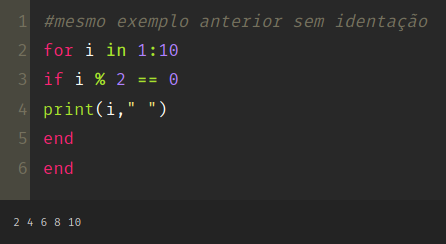
\includegraphics[width=12cm]{aplicacoes/identacao.png} \\
%        {\tiny \sf Fonte: Autor}
%    \end{center}
%    \end{figure} 
 
    \begin{figure}[H]%supressao
    \begin{center}
        \label{supressao}
        \caption{Supressão de output em REPL} %\label{REPL}
        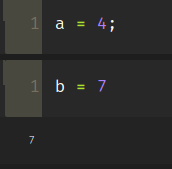
\includegraphics[width=6cm]{aplicacoes/supressao.png} \\
        {\tiny \sf Fonte: Autor}
    \end{center}
    \end{figure} 

    \begin{figure}[H]%emoji
      \begin{center}
        \label{emoji}
        \caption{Unicode nos nomes de variável} 
        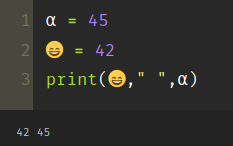
\includegraphics[width=6cm]{aplicacoes/emoji.png} \\
        {\tiny \sf Fonte: Autor}
    \end{center}
    \end{figure} 

    \begin{figure}[H]%indice
    \begin{center}
        \label{indice}
        \caption{Indices em Julia iniciam na posição 1} 
        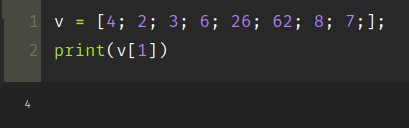
\includegraphics[width=12cm]{aplicacoes/indice.png} \\
        {\tiny \sf Fonte: Autor}
    \end{center}
    \end{figure} 

    \begin{figure}[H]%exclamacao
    \begin{center}
      \label{exclamacao}
      \caption{Diferença entre as funções sort() e sort!()} 
        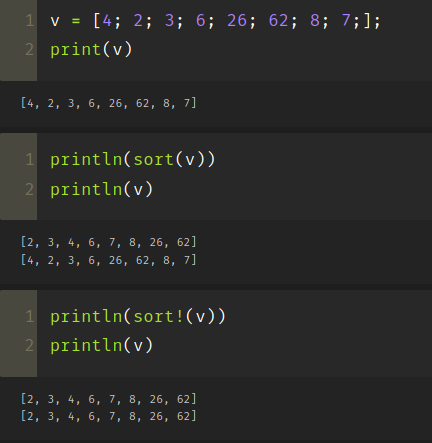
\includegraphics[width=12cm]{aplicacoes/exclamacao.png} \\
        {\tiny \sf Fonte: Autor}
    \end{center}
    \end{figure} 

\section{Pacotes e módulos}

Os criadores da lingua escolheram construir um núcleo leve complementado por uma biblioteca padrão (Standard Library) distribuída junto dos binários, e um poderoso gerenciador de pacotes capaz de baixar (muitas vezes direto de repositórios GitHub), pré compilar, atualizar e resolver dependências de pacotes a partir de comandos simples. 

Para acessar o gerenciador de pacotes podemos importar o módulo de pacotes (import Pkg) e executar os comandos no formato Pkg.(ARGS). Demonstramos esse caso de uso na figura \ref{import_Pkg} onde executamos o comando para instalar o pacote Plots. Como o pacote já está instalado, o Pkg apenas o reconhece e não altera os pacotes.
%A figura \ref{import_Pkg} demonstra esse caso de uso ao tentarmos instalar o pacote Plots que como já está instalado, podemos observar que o Pkg reconhece tal fato e não altera nossos pacotes. 
Também podemos utilizar o modo especial de pacotes no REPL que traz algumas facilidades como autocompletar por exemplo. Nesse caso, basta digitar "]" para entrar nesse modo especial do REPL, como mostrado na figura \ref{pkg}. Na figura \ref{REPL_plots} repetimos o comando para instalar a biblioteca Plots, dessa vez no REPL. 
%Já no REPL também podemos apenas digitar ] para entrar no modo especial de pacotes, conforme a figura \ref{pkg}. nele temos algumas facilidades como autocomplete.
\begin{figure}[H]
\begin{center}
    \caption{Utilizando o Pkg em scripts} \label{import_Pkg}
    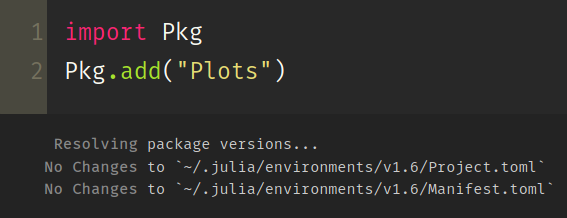
\includegraphics[width=12cm]{aplicacoes/import_Pkg.png} \\
    {\tiny \sf Fonte: Autor}
\end{center}
\end{figure} 

\begin{figure}[H]
\begin{center}
    \caption{REPL - modo pacotes} \label{pkg}
    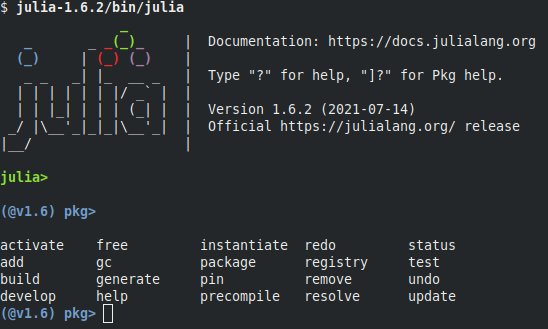
\includegraphics[width=12cm]{aplicacoes/pkg.png} \\
    {\tiny \sf Fonte: Autor}
\end{center}
\end{figure} 

\begin{figure}[H]
\begin{center}
    \caption{Utilizando modo Pkg do REPL } \label{REPL_plots}
    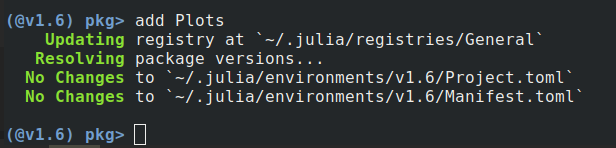
\includegraphics[width=12cm]{aplicacoes/REPL_plots.png} \\
    {\tiny \sf Fonte: Autor}
\end{center}
\end{figure}

Listamos a seguir alguns dos principais comandos do módulo Pkg. Em seguida demonstramos exemplos com o comando "status"  tanto no modo especial de pacotes do REPL (figura \ref{pacotes}) quanto em um exemplo de código Julia (figura \ref{Pkg_script}):
\begin{itemize}
  \item \textbf{status:} retorna uma lista (nome e versão) dos pacotes instalados localmente.
  \item \textbf{update:} atualiza o índice local de pacotes e os próprios pacotes para a versão mais recente.
  \item \textbf{add nomePacote:} automaticamente baixa e instala um pacote.
  \item \textbf{rm nomePacote:} remove o pacote e todas as suas dependências.
\end{itemize}

\begin{figure}[H]
\begin{center}
    \caption{Pkg.status no modo de pacotes do REPL} 
    \label{pacotes}
    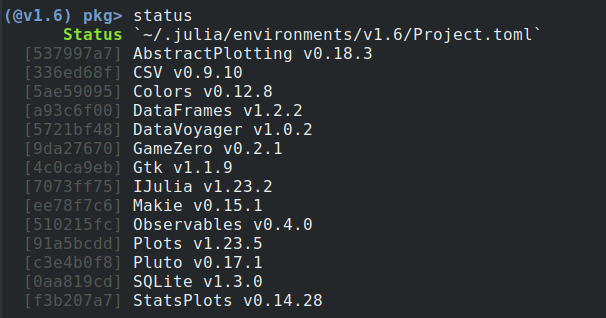
\includegraphics[width=12cm]{aplicacoes/pacotes.png} \\
    {\tiny \sf Fonte: Autor}
\end{center}
\end{figure} 
\begin{figure}[H]
\begin{center}
    \caption{Pkg.status em código Julia} 
    \label{Pkg_script}
    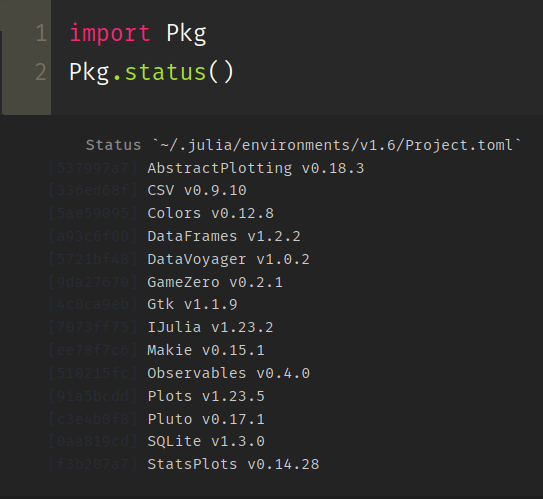
\includegraphics[width=12cm]{aplicacoes/Pkg_script.png} \\
    {\tiny \sf Fonte: Autor}
\end{center}
\end{figure} 

Uma vez instalado, para utilizar um pacote devemos utilizar um dos comandos seguintes:
\begin{itemize}
  \item \textbf{use:} permite acessar diretamente as funções de um pacote, basta adicionar o comando (using nomePacote) no inicio do script. 
  \item \textbf{import:} tem a mesma funcionalidade do use com a diferença de precisarmos nos referir ao nome completo da função (nomePacote.nomeFunção), o que tem a vantagem de manter a organização dos nomes. Via de regra, nesse caso definimos apelidos para os pacotes como por exemplo chamar o "Plots" de "pl" (const pl = Plots) %adicionar exemplo de código? []
\end{itemize}

%%Da mesma forma podemos usar (\textbf{use}) ou importar (\textbf{import}) qualquer arquivo Julia como módulo. Ele será analogamente executado ao ser invocado e qualquer símbolo definido estará disponível no escopo onde foi chamado. 

\section{Sistema de ajuda}
Além do sistema de pacotes, basta digitar "?"  para acessar o modo especial de ajuda do REPL. Assim, acordo com a documentação do termo buscado o sistema de ajuda pode retornar sua lista de métodos, exemplos de uso, descrição, lista de argumentos ou termos ou ainda os termos relacionados, conforme podemos ver na figura \ref{ajuda}. 
    \begin{figure}[H]
    \begin{center}
        \caption{REPL - modo ajuda} \label{ajuda}
        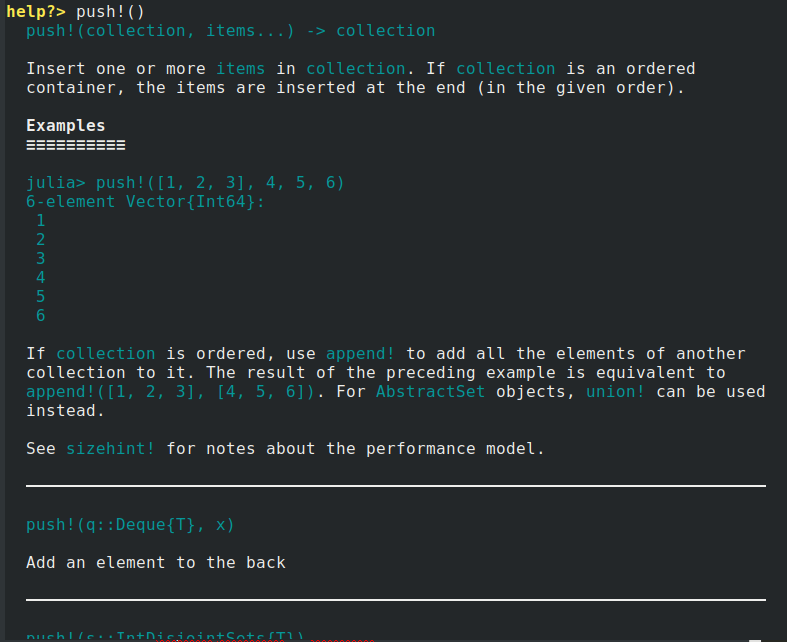
\includegraphics[width=12cm]{aplicacoes/help.png} \\
        {\tiny \sf Fonte: Autor}
    \end{center}
    \end{figure} 
%a linguagem também oferece um sistema de ajuda que retorna informação sobre o uso da maior partes das funções que pode ser acessado no REPL digitando "?" ou através do comando "?{termo de busca}". 

\section{Tipos e estruturas de dados}
Segundo \cite{Lobianco2019}, Julia oferece nativamente um sistema hierárquico e bastante completo de tipos predefinidos que são divididos entre \textbf{escalares} e \textbf{coleções}.
Escalares são tipos atômicos, indivisíveis, como por exemplo inteiros, floats, e chars. Já as coleções são objetos que acomodam outros objetos como por exemplo vetores multidimensionais, dicionários e conjuntos.

Nesse sentido, podemos destacar as seguintes características: 
\begin{itemize}
    \item Cada valor (mesmo os primitivos) tem seu tipo único, por convenção iniciando com letra maiúscula como Int64 e Bool (fig \ref{tipos_escalares}). 
    \item Na hierarquia dos tipos, o mais amplo é o tipo genérico Any.
    \item No caso de coleções e alguns escalares, o nome de seu tipo é seguido de chaves indicando os tipos dos elementos contidos, e sua dimensão, como por exemplo Array\{Int64,1\}, normalmente chamado de Vector\{Int64\}, ou seja uma coleção unidimensional de elementos do tipo Int64 como mostra a figura \ref{tipos_parametricos}. Na terminologia da linguagem são chamados tipos paramétricos.  
    \item Em Julia não existe divisão entre objetos e não-objetos pois todos os valores são objetos tipados, enquanto variáveis são apenas nomes relacionados a valores, portanto não têm tipo. 
   % \item Objetos do tipo coleção podem são denominados imutáveis quando não é possível alterar o seu valor (e valor de seus elementos), 
    \item Podemos converter objetos atraves da função "convert(T,x)", ou passar o objeto como argumento para uma função do tipo no formato "T(x)" como "Int64(x)" por exemplo, conforme a figura \ref{conversao} demonstra. 
    \item O operador :: pode ser utilizado para anexar anotações de tipo para expressões e variáveis conforme a figura \ref{anotacao_tipo}. \cite{Bezanson2017} afirma que essa anotação manual de tipos é totalmente opcional, pois apesar de haver situações nas quais ela se traduz em algum ganho de performance, na imensa maioria dos casos a inferência de tipos é suficiente para atingir eficiência máxima na compilação. Ainda assim a anotação de tipos é frequentemente utilizada para confirmar que um programa se comporta conforme o esperado. 
    
\end{itemize}


    \begin{figure}[H]
    \begin{center}
        \caption{Tipos escalares de dados} \label{tipos_escalares}
        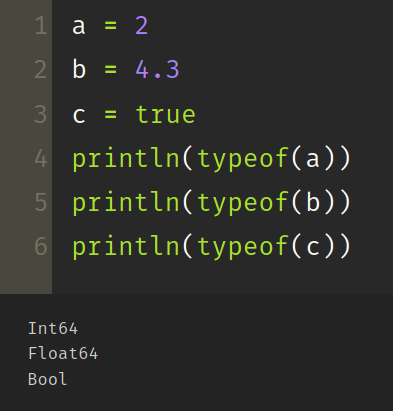
\includegraphics[width=10cm]{aplicacoes/tipos_simples.png} \\
        {\tiny \sf Fonte: Autor}
    \end{center}
    \end{figure} 

    \begin{figure}[H]
    \begin{center}
        \caption{Tipos paramétricos de dados} \label{tipos_parametricos}
        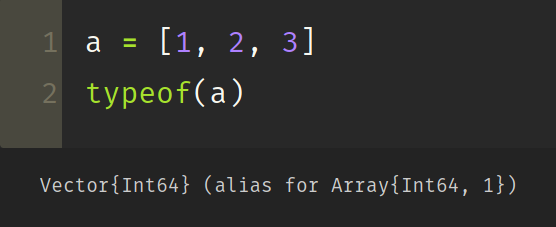
\includegraphics[width=12cm]{aplicacoes/tipos_parametricos.png} \\
        {\tiny \sf Fonte: Autor}
    \end{center}
    \end{figure}

    \begin{figure}[H]
    \begin{center}
        \caption{Conversão de tipos} \label{conversao}
        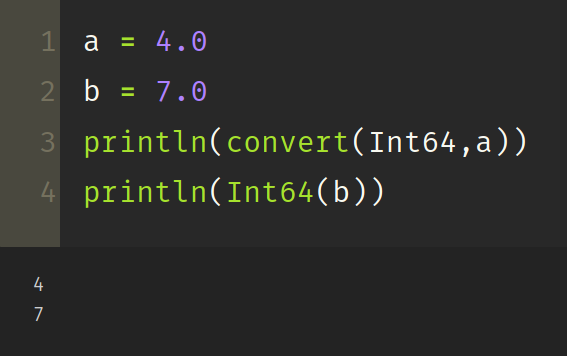
\includegraphics[width=12cm]{aplicacoes/convert.png} \\
        {\tiny \sf Fonte: Autor}
    \end{center}
    \end{figure}


    \begin{figure}[H]
    \begin{center}
        \caption{Anotação de tipos} \label{anotacao_tipo}
        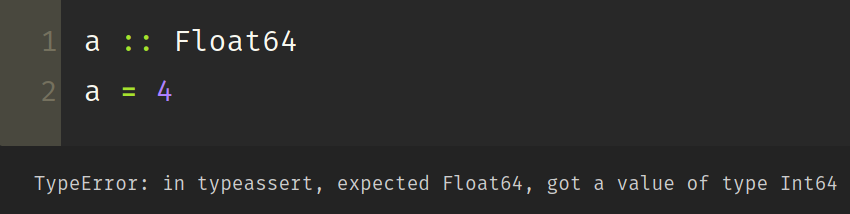
\includegraphics[width=12cm]{aplicacoes/type_annotation.png} \\
        {\tiny \sf Fonte: Autor}
    \end{center}
    \end{figure} 

    \subsection{Tipos simples}
    \begin{itemize}
      \item Caracteres individuais são do tipo Char, e representado por aspas simples.
      \item Booleanos são do tipo Bool, apenas com as instâncias True e False. Em um contexto de inteiros, booleanos podem ser interpretados como 0 e 1, assim como os inteiros 0 e 1 podem ser interpretados como booleanos, conforme é demonstrado na figura \ref{bool}.  
      %porém o oposto não ocorre (if 0 gera o erro de tipo "non-Boolean used in Boolean context"
    \item O tipo padrão de inteiro é o Int64 (existem outros 9 tipos inteiros) capaz de armazenar valores entre $-2^{63}$ e $2^{63-1}$.
    \item De modo análogo o padrão de ponto flutuante é o Float64.
    \item Números complexos são suportados pela variável global im que representa a raiz quadrada de -1 (fig \ref{complex}).
  \end{itemize}
 
    \begin{figure}[H]
    \begin{center}
        \caption{Tipo Bool} \label{bool}
        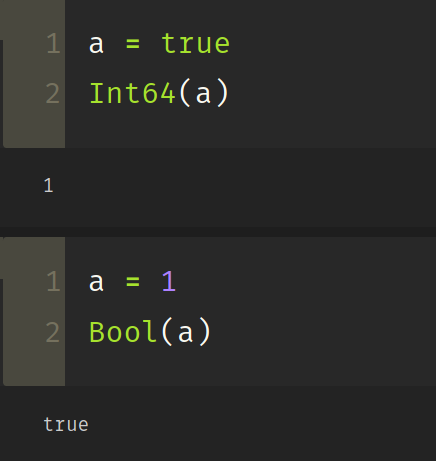
\includegraphics[width=12cm]{aplicacoes/bool.png} \\
        {\tiny \sf Fonte: Autor}
    \end{center}
    \end{figure} 

  \begin{figure}[H]
  \begin{center}
      \caption{Números complexos} \label{complex}
      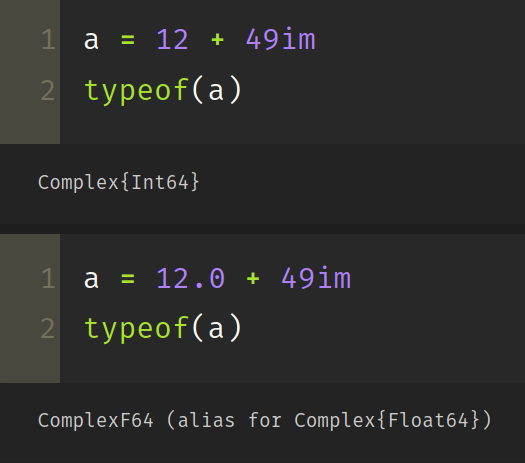
\includegraphics[width=12cm]{aplicacoes/complex.png} \\
      {\tiny \sf Fonte: Autor}
  \end{center}
  \end{figure} 

\subsection{Operações básicas}
Além dos operadores padrões de soma, subtração, multiplicação e divisão (+, -, *, /) temos a potenciação através do circunflexo ("3\^{}2"), a raiz quadrada por meio da função "sqrt()", o resto pelo operador \%, e a divisão inteira pelo símbolo $\div$ ("\textbackslash div" + tab), conforme apresentamos na figura \ref{operacoes}. 

    \begin{figure}[H]
    \begin{center}
        \caption{operacoes} \label{operacoes}
        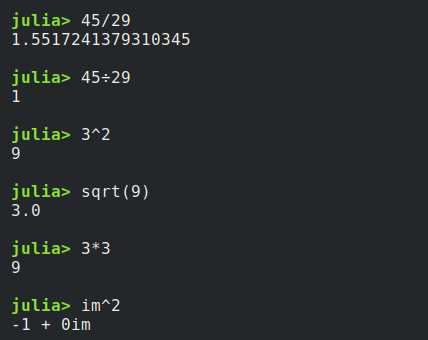
\includegraphics[width=12cm]{aplicacoes/operacoes_basicas.png} \\
        {\tiny \sf Fonte: Autor}
    \end{center}
    \end{figure} 



\subsection{Arrays}
Arrays (Array\{T, N\}) são coleções de N dimensões. %Isto é, um array acomoda elementos em ordem 
 Eles podem conter elementos de apenas um tipo (T), sendo que T pode ser de algum dos tipos que já abordamos, ou dos tipos especiais Any ou Union{}. O tipo genérico Any tem a vantagem de permitir arrays heterogêneos, entretanto, de acordo \cite{Lobianco2019}, Array(Any,N) são consideravelmente menos performáticos que arrays homogêneos, pois no caso dos homogêneos, e até mesmo do tipo Union\{$T_1,...,T_n$\}, o compilador da linguagem é capaz de gerar código mais específico e otimizado para os tipos em questão, o que não é possível para o tipo Any.  
 %heterogêneos -nesse caso tendo o tipo genérico (Any) que em geral é consideravelmente menos performático- ou ser do tipo união (Union\{$T_1,T_2$\}) de outros tipos (exemplo: Union\{Int64,String\}), que consegue ter performace próxima do monotipo a partir dessa restrição.

 Alguns tipos de arrays recebem nomes especiais como por exemplo os vetores (Vector\{T\}) que são vetores unidimensionais, as matrizes (Matrix\{T\}) que são vetores bidimensionais e as Strings que são ainda um subtipo de vetor de caracteres. 

%Além das Strings que são vetores imutáveis de caractéres, também temos os tipos especiais Vector\{T\} e Matrix\{T\} que são respectivamente Arrays de uma e duas dimensões.

\subsubsection{Criação de Array}
Existem diversas formas de criarmos um Array do tipo T:
\begin{lstlisting}
     a  = [1;2;3] #cria um vetor coluna de uma dimensao.
     a = [1 2 3] #cria um vetor linha de uma dimensao.
     a = [] #cria um Array{Any,1}
     a = Int64[] #constroi um vetor de Int64 com uma dimensao.
     a = Array{Int64,1}() #mesmo do anterior, usando construtor.
     a = zeros(n) #cria um Array{Float64,1}
     a = zeros(Int64,n) #cria um array do tipo Int64 com n zeros.
     a = fill(j,n) #vetor com n elementos j
     a = rand(n) #vetor preenchido com n numeros aleatorios
\end{lstlisting}

\subsubsection{Acessar elementos}
Podemos acessar subvalores de um array utilizando chaves para selecionar um elemento (a[2]) ou uma fatia de intervalo fechado (a[de:passo:até]) da seguinte forma:
\begin{lstlisting}
   a = [1 2 3 4 5 6 7] 
   a[4] #retorna 4
   a[1:3] #retorna os elementos 1,2,3
   a[1:2:end] #retorna 1 3 5 7
   a[end:-1:1] #retorna 7 6 5 4 3 2 1
\end{lstlisting}

\subsubsection{Principais funções}
A seguir apresentamos as principais função para trabalharmos com Arrays, é interessante notar que normalmente as funções que podem modificar algum de seus argumentos contém uma exclamação.
\begin{lstlisting}
  push!(a,b) #adiciona o elemento b no fim de a.
  append!(a,b) #adiciona os elementos de b em a,
  #identico ao push! caso b seja escalar

  c = vcat(1,[2,3],[4,5]) #concatena arrays

  pop!(a) #remove o ultimo elemento do array,
  popfirst!(a) #remove o primeiro elemento do array.
  deletat!(a,pos) #remove o elemento da posicao pos

  pushfirst!(a,b) #b no inicio de a.

  length(a) #=ou=# if a in b end #retorna o comprimento do vetor

  sort!(a) #ordena o vetor a.
  sort(a) #retorna a ordenado sem modificar o vetor original
  reverse(a) #retorna elementos de a invertidos

  unique!(a) #remove duplicatas modificando a.
  unique(a) #retorna a sem duplicadas. 
  in(b,a) #checa a existencia de b em a.

  a... #=operador "splat" coverte os elementos em 
  parametros para uma funcao.=#

  maximum(a) #=ou=# max(a...) #retorna o maior valor.
  minimum(a) #=ou=# min(a...) #analogo ao anterior.
  sum(a) #retorna a soma dos elmentos de a.
  cumsum(a) #retorna um vetor com a soma cumulativa de a.

  empty!(a) #esvazia um vetor coluna.
  b = vec(a) #transforma vtores linha em vetores coluna.
  shuffle(a) #=ou=# shufle!(a) #=embaralha aleatoriamente 
  os elementos de a.=# 
  (requer o modulo Random).=#

  isempty(a) #checa se um array esta vazio.

  findall(x ->  x == value, a) #=retorna o indice de todas
  as ocorrencias de x.=#
  deleteat!(a, findall(x ->  x == value, a)) #=deleta todas as 
  ocorrencias de x de a.=#

  enumerate(a) #retorna um iterador de pares (indice, elemento).
  zip(a,b) #retorna um iterador de pares (a_element,b_element).
\end{lstlisting}

\subsubsection{Arrays aninhados e multidimensionias}
Arrays multidimencionais são os objetos do tipo Array\{T,N\} sendo o número de dimenções N maior que um, enquanto Arrays Aninhados apresentam uma dimensão sendo pelo menos um de seus elementos outro Array, como por exemplo um vetor de vetores Array\{Array\{T,1\},1\}.

A principal diferença entre ambos é que em matrizes o número de elemento em cada coluna deve ser igual e as regras da Álgebra Linear são aplicáveis. 


Os elementos de Arrays aninhados podem ser acessados por chaves duplas (a[2][3]), Já os elementos de multidimensionais podem ser acessados com os índices de cada dimensão separados por vírgula (a[lin,col]). Para vetores colunas tanto a[2] quanto a[1,2] retornam o segundo elemento. 

Podemos contruir Arrays multidimensionais de modo análogo aos vetores, alias estes são um caso específico daqueles:
\begin{lstlisting}
  a = [[1,2,3] [4,5,6]] #cria por colunas
  a = [1 4; 2 5; 3 6] #cria por linhas
  a = zeros(In64,n,m,g) #=cria uma matriz nxmxg 
  preenchida com zeros.=#
  a = [3x + 2y + z for x in 1:2, y in 2:3, z in 1:2] 
  #=tambem podemos usar list comprehension.=#
\end{lstlisting}

Também temos funções particularmente úteis para trabalharmos com Arrays multidimencionais:
\begin{lstlisting}
  size(a) #retorna uma tupla com os damanhos de cada dimencao
  ndimns(a) #retorna o numero de dimensoes.
  reshape(a,nElementDim1, nElementsDim2,...,nElementDimN) 
  #redimensiona o array.
  dropdimns(a, dimns=(dimRemov1, dimRemov2) 
  #remove as dimensoes especificadas
  transpose(a) #=ou=# a' #transpoe vetores ou matrizes.
  hvat(col1,col2) #concatena horizontalmente
  vcat(row1, row2) # concatena verticalmente. 
\end{lstlisting}
\subsection{Strings}
As strings (String) em Julia são vetores imutáveis de caracteres, isto é: conforme apresentamos na figura TAL, não é possível alterar nenhum dos elementos de uma String. 
Elas são definidas com aspas duplas e podem ser vistas como um tipo especial de vetor pois suportam indexação e looping.


Algumas das operações típicas com strings são:
\begin{itemize}
    \item \textbf{split(s, " ")} nesse exemplo utiliza o espaço como um separador e retorna um vetor com as sublistas.
    \item \textbf{join([s1,s2], " ")} que une strings utilizando, nesse caso, o espaço entre cada junção.
    \item \textbf{replace(s, {termo buscado}} =  {substituto}) que substitui substrings compatíveis com a busca.
    \item parse(Int, "64") retorna a string convertida para um tipo numérico, no caso inteiro.
    \item \textbf{string(123)} retorna a string correspondente ao número.
    \item Existem três principais maneiras de concatenar strings:
        \subitem 
        \begin{lstlisting}    
  string("Hello, ","world")
  "Hello, World! The answer is $(43)"
  "Hello, " * "world"
        \end{lstlisting}
        
\end{itemize}



\subsection{Tuplas e Tuplas Nomeadas}
Tuplas (Tuple\{T1, T2,...\}) são listas imutáveis de elementos, que em contraste com Arrays não perdem performace ao conter elementos de tipos diversos porque suas assinaturas são mantidas. Podmos criar tuplas com parênteses ou sem conforme o exemplo:
\begin{lstlisting}
  t = (1, 2.5, "a")
  t = 1, 2.5, "a"
#Podemos converter uma tupla em um array:
  a = [t...] #utilizando o operador splat
  a = [i[1] for i in t] #utilizando list comprehension
  a = collect(t) #utilizando o operador collect. 
#De modo analogo podemos converter um array em uma tupla:
  t = (a...,)
\end{lstlisting}  
%\subsection{Tuplas nomeadas}
Já as Tuplas Nomeadas (NamedTuple) são coleções de itens que além do índice seus elementos podem ser identificados pelo nome da seguinte forma: 
\begin{lstlisting}
  nt = (a=1,b=2.5) #define uma tupla nomeada
  nt.a #acessa o elemento a da tupla nt.
  keys(nt) #returna uma tupla com os nomes: (a,b)
  values(nt) #retorna uma tupla com os valores: (1, 2.5).
  collect(nt) #retorna um array com os valores.
  pairs(nt) #retorna um iterador dos pares (nome,valor) 
\end{lstlisting}

\subsection{Dicionários}
Dicionários (Dict\{Tkey, Tvalue\}) guardam mapas de chaves para valores com ordem aparentemente aleatória e diferente das Tuplas nomeadas, são mutáveis, tipo-instáveis.
Os principais métodos para trabalharmos com dicionários são:
\begin{lstlisting}
  d = Dict() 
  #cria um dicionario vazio.
  d = Dict{String,Int64}() 
  #cia um dicionario com tipagem definidapara chaves e valores.
  d = Dict('a'= 1,'b'= 2, 'c'= 3) 
  #inicializa o dicionario com valores
  d[novaChave] = novoValor 
  #adiciona um novo par key-value ao dicionario.
  delete!(d,"chave") 
  #deleta o par correspondente a chave.
  map( (i,j) -  d[i]=j, ['a','b','c'],[1, 2 , 3]) 
  #adiciona pares de mapeamentos
  d["chave"] 
  #=retorna o valor correspondente a chave, 
  ou um erro caso ela nao exista.=#
  get(d, 'chave', "Chave inexistente") 
  #=retorna o valor da chave ou um valor padrao 
  caso ela nao exista.=# 
  keys(d) #retorna um iterator com todas as chaves de d.
  values(d) #retorna um iterador com todos os valores de d.
  haskey(d,"chave") 
  #retorna um booleano de acordo com a existencia da chave.
  in(('a'= 1), d) 
  #=checa se o par existe e a chave corresponde 
  ao valor especificado.=#

\end{lstlisting}

\subsection{Sets}
Usamos sets (Set\{t\}) para representar conjuntos mutáveis e sem ordem de valores únicos.
    \begin{lstlisting}
          s = Set() #=ou=# Set{T}() 
        #cria um set vazio
          s = Set([1,2,2,3,4]) 
        #inicializa com valores desconsiderando o 2 duplicado
          push!(s,5) 
        #adiciona elementos
          delete!(s,1)
        #deleta elementos
          intersect(s1,s2) 
        #intersessao de s1 e s2
          union(s1,s2) 
        #uniao de s1 e s2
          setdiff(s1,s2) 
        #diferenca entre s1 e s2
    \end{lstlisting}

\subsection{Números aleatórios}
Julia também facilita a obtenção de números pseudo aleatórios:
    \begin{lstlisting}
  rand()  
#retorna um float entre 0 e 1
  rand(a:b) 
#retorna um inteiro no intervalo [a,b]
  rand(a:0.01:b) 
#float aleatorio com precisao no segundo digito

#=Tambem podemos obter numeros de alguma distribuicao particular, 
desde que usemos o pacote Distributions=#

  rand(nomeDistribuicao[parametros])
  rand(Uniform(a,b))#por exemplo

#=Igualmente importante e a definicao da semente pseudo aleatoria
que permite termos um script reprodutivel:=#
  Random.seed!(1234) 
#define a semente pseudo-aleatoria para 1234
  Random.seed!() 
#reseta a definicao da semente

  rand(Uniform(a,b),2,3) 
#uma matriz 2x3 de numeros uniformemente aleatorios no 
intervalo [a,b].

    \end{lstlisting}
\subsection{Valores Faltantes}
Julia suporta diversos conceitos de falta:
\begin{itemize}
    \item \textbf{nothing} (tipo Nothing) é o valor utilizado para blocos e funções que retornam nada. Conhecido como "null do engenheiro de software"
    \item \textbf{missing} (tipo Missing) representa um valor faltante no sentido estatístico, em que deveria haver um valor, apenas o desconhecemos. De modo que os containers e maioria das operações conseguem lidar eficientemente com esses casos. Também conhecido como "null do cientista de dados"
    \item \textbf{Nan} (tipo Float64) representa o resultado de uma operação que retorna é um "não-número". Similar ao missing no sentido de se propagar silentimente ao invés de gerar um erro. Analogamente Julia também oferece Inf (1/0) e -Inf (-1/0).
\end{itemize}
\section{Controle de fluxo e funções}
Em Julia nos temos as principais estruturas condicionais e repetitivas que encontramos nas linguagens mais populares.
\subsection{Estrutura em bloco}
A sintaxe do controle de fluxo tipicamente se dá atráves de blocos que se iniciam com uma palavra chave seguida de uma condição (com parêntesis opcionais), e finalizam com a palavra "end" da seguinte forma: 
    \begin{lstlisting}
    <palavra chave>  <condicao> 
        #... conteudo do bloco....
    end 
    #-----------------------------#
    #Por exemplo:
    for i in 1:5
        print(i)
    end     
    \end{lstlisting}

\subsection{Iteração repetida}
\subsubsection{For e while}
As funções for e while em Julia são muito flexíveis, soportando os contrutos padrões como percorer vetores, break que imediatamente aborta uma sequência e continue que imediatamente pula para a próxima iteração. Além de suportar condições múltiplas como demonstrado no exemplo abaixo. 
\begin{lstlisting}
for i=1:2, j=2:5
	println("i:$i, j:$j")
end
#=temos condicoes multiplas que geram um 
loop aninhado onde j percorre o intervalo 2:5 
para cada elemento i.=#

for i in "string exemplo"
	println(i)
end 
\end{lstlisting}
\subsubsection{List comprehension}
List comprehension é essencialmente uma forma compacta de escrever um loop:
\begin{lstlisting}
a = [f(i) for i in [1 2 3]] 
#cria um array com f aplicada a cada elemento de [1 2 3]

[x+2y for x in [10,20,30], y in [1,2,3]]

[d[i]=value for (i,value) in enumerate(lista)

[estudantes[nome] = idade for (nome,idade) in zip(nomes,idades)]
\end{lstlisting}
\subsubsection{Map}
Já a função Map aplica uma função a uma lista de argumentos.
\begin{lstlisting}
map((nome,idade) -  estudantes[nome] = idade, nomes, idades)

a = map(f, [1,2,3]) 

a = map(x- f(x), [1,2,3])
\end{lstlisting}

\subsection{Condicionais}
Condicionais também são estruturados seguindo o design de simplicidade e similaridade com as linguagens dinâmicas:
\begin{lstlisting}
i = 5
if i == 1 
	println("i = 1")
elseif i == 2
	println("i = 2")
else 
	println("i nao e nem 1 nem 2")
end
\end{lstlisting}

As expressões são avaliadas até que seja possível inferir seu resultado (short circuited).%[] Pesquisar quão comun isso é

Assim como list comprehension é uma forma concisa de escrever um loop temos no operador ternário uma forma concisa de escrever um condicional:
\begin{lstlisting}
a? b: c
#se a eh verdadeiro execute b, do contrario execute c
\end{lstlisting}

\subsection{Funções}
Funções em Julia são muito flexíveis, podem ser delfinadas tanto em linha como em bloco quanto como funções lambda. Além disso, funções também são objetos, e portanto podem ser atribuídas a novas variáveis, retornadas como valores ou aninhadas:
\begin{lstlisting}
  f(x,y) = 2x+y
#definicao em uma linha
#-------------
  function f(x) 
  	2x + y 
  end
#definicao em bloco
#--------------
  x,y -  2x + y
#funcao anonima
#--------------
  a = f
  a(5)
#funcao como objeto
\end{lstlisting}

A chamada de funções em Julia seguem uma convenção conhecida como chamada por compartilhamento, que seria entre chamada por referência (onde um ponteiro a memória da variável é passado) e chamada por valor (onde uma cópia da variável é passada e a função trabalha nessa cópia).

Assim, as funções em Julia trabalham nas novas variáveis locais, conhecidas apenas dentro da função, de modo que atribuir a variável a outro objeto não vai influenciar o valor original, mas se o objeto ligado a variável é mutável a mutação do objeto também será aplicada a variável original:
\begin{lstlisting}
  function f(x,y) 
  	x = 10
  	y[1] = 10
  end
  x = 1
  y = [1,1]
  f(x,y)
#Resultado: x = 1, y = [10, 1]

\end{lstlisting}

Na comunidade Julia se recomenda seguir duas regras em relação a funções:%%[] ler no livro pra melhorar a coesão 
\begin{itemize}
    \item Que contenham todos os elementos necessários para sua lógica (sem acesso a nenhuma variável exceto seus parâmetros e constantes globais.)
    \item Que não alterem nenhuma outra parte do programa, ou seja, que não produza nenhum efeito colaterial além da eventual modificação de algum de seus argumentos. 
\end{itemize}

\subsubsection{Argumentos}
\begin{itemize} %%[] Adicionar exemplos em códigos
    \item Normalmente os argumentos são posicionais, mas temos o operador ponto e vírgula (;) para estabelecer que após o mesmo todos os argumentos sejam especificados por nome (keywords arguments)
    \item Os últimos argumentos podem ser especificados junto com valores padrão.
    %\item Também podemos declarar uma função de múltiplos argumentos.
    \item Funções podem receber um número variável de argumentos. 
    \item Também temos a opção de especificar os tipos dos argumentos. Como mencionado, a principal razão para limitar os tipos dos parâmetros é para evidenciar possíveis bugs logo no início caso uma função seja acidentalmente chamada com um tipo diferente do planejado, retornando um erro de tipo ao invés de silentemente continuar a execução.
    \item Retornar um valor é opcional e normalmente as funções retornam o último valor computado, podendo ser inclusive uma tupla.
\end{itemize}
\begin{lstlisting}
  f(a,b=1;c=2) = (a+b+c) 
  f(1,c=3) 
#(1+1+3)

  function f(args...)
  	for arg in args
  		println(arg)
  	end
  end

  f(a::In64, b::Int64, c::Int64) = (a+b+c)

  f(a,b) = a*2,b+2
  x,y = f(1,2) 
# x = 2, y = 4
    
\end{lstlisting}

%\subsubsection{Multiple-Dispatch}
%Uma função pode ter múltiplos métodos para diferentes números e %tipos de inputs. Ao ser executada o computador selecionará a %implementação correta de acordo com os parâmetros na chamada da %função. Podemos listar todos os métodos de uma função com a função %methods(f).
%%Detalhar mais esse que é o coração da linguagem